%\usepackage[round,colon,authoryear]{natbib}

\chapter{Querying bacterial genomes with transposon-insertion sequencing}
\label{sec:chapter_piRNAs}
\ifpdf
    \graphicspath{{Chapter1/Chapter1Figs/PNG/}{Chapter1Chapter1Figs/PDF/}{Chapter1/Chapter1Figs/}}
\else
    \graphicspath{{Chapter1/Chapter1Figs/EPS/}{Chapter1/Chapter1Figs/}}
\fi


\textit{This chapter is an expansion of the previously published article ``Approaches to querying bacterial genomes using transposon-insertion sequencing'' \parencite{Barquist2013}. Amy K. Cain and Christine J. Boinett (Pathogen Genomics, Wellcome Trust Sanger Institute) contributed to the research of the original article. All final language is my own.}

\section{Introduction}

A common approach to identifying genomic regions involved in survival under a particular set of conditions is to screen large pools of mutants simultaneously. This can be done with defined mutants \parencite{Baba2006, Hobbs2010}; however, the construction of defined mutant libraries is labor-intensive and requires accurate genomic annotation, which can be particularly difficult to define for non-coding regions. An alternative to defined libraries is the construction and analysis of random transposon-insertion libraries. The original application of this method used DNA\nomenclature[Z]{DNA}{Deoxyribonucleic acid} hybridization to track uniquely tagged transposon-insertions in {\it Salmonella enterica} serovar Typhimurium over the course of BALB/c\nomenclature[Z]{BALB}{Bagg albino (mouse)} mouse infection \parencite{Hensel1995}. DNA hybridization was eventually superseded by methods that used microarray detection of the genomic DNA flanking insertion sites, variously known as TraSH\nomenclature[Z]{TraSH}{Transposon site hybridization}, MATT\nomenclature[Z]{MATT}{Microarray tracking of transposon mutants}, and DeADMAn\nomenclature[Z]{DeADMAn}{Designer microarrays for defined mutant analysis} (reviewed in \cite{Mazurkiewicz2006}). However, these methods suffered from many of the problems microarrays generally suffer from: difficulty detecting low-abundance transcripts, mis-hybridization, probe saturation, and difficulty identifying insertion sites precisely.

The application of high-throughput sequencing to the challenge of determining insertion location and prevalence solves many of these problems. Interestingly, the first application of transposon-insertion sequencing, developed by \textcite{Hutchison1999}, actually predates the development of microarray-based methods. However, this was applied to libraries of only approximately 1000 transposon mutants in highly reduced {\it Mycoplasma} genomes, and the difficulty of sequencing at the time prevented wide spread adoption or high resolution. Modern high-throughput sequencing technology allows the methods discussed in this chapter to routinely monitor as many as one million mutants simultaneously in virtually any genetically tractable microorganism. 

% Table generated by Excel2LaTeX from sheet 'Sheet1'
%
\begingroup
\begin{landscape}
   \tiny
   \noindent
    \begin{longtable}{ l
    				l
				l
				l
				p{2in}
				l
				l}
    \caption[Summary of transposon-insertion sequencing studies to date]{A collection of studies to date utilizing transposon-insertion sequencing. Columns: 1) study reference,  2) organism mutagenized, 3) number of mutants generated, 4) insertion density, 5) brief description of the application, 6) transposon used, 7) method name coined, if any.}
    \\
    \toprule
    \textbf{Study} & \textbf{Organism} & \textbf{Total Mutants} & \textbf{Density} & \textbf{Application} & \textbf{Tn used } & \textbf{Name Coined} \\
    \midrule
    \multirow{2}[1]{*}{\textcite{Hutchison1999}}  & \multirow{2}[1]{*}{\textit{M. genitalium}} & 1291  &  ~1/850 bp & \multirow{2}[1]{2in}{Required gene sets} & \multirow{2}[1]{*}{Tn4001} & \multirow{2}[1]{*}{GTM\nomenclature{GTM}{Global transposon mutagenesis} } \\
          &  \textit{M. pneumoniae}     & 918   & ~1/850 bp &       &       &  \\
    \multirow{2}[0]{*}{\textcite{Goodman2009}} & \multirow{2}[0]{*}{\textit{B. thetaiotaomicron}} & \multirow{2}[0]{*}{2 X 35,000} & \multirow{2}[0]{*}{1/182 bp} & \multirow{2}[0]{2in}{Establishment in human gut as a natural habitat} & \multirow{2}[0]{*}{Mariner} & \multirow{2}[0]{*}{INSeq} \\
          &       &       &       &       &       &  \\
    \multirow{2}[0]{*}{\textcite{Gawronski2009} } & \multirow{2}[0]{*}{\textit{H. influenzae}} & \multirow{2}[0]{*}{75,000} & \multirow{2}[0]{*}{1/32 bp} & \multirow{2}[0]{2in}{Prolonged survival in lung in vivo} & \multirow{2}[0]{*}{Mariner} & \multirow{2}[0]{*}{ HITS} \\
          &       &       &       &       &       &  \\
   \textcite{Opijnen2009}  & \textit{S. pneumoniae} & 6 x 25,000 & 1/91bp & Transcriptional regulation and carbohydrate transport & Mariner & Tn-seq \\
    \multirow{2}[0]{*}{\textcite{Langridge2009a}}  & \multirow{2}[0]{*}{{\it S.} Typhi1} & \multirow{2}[0]{*}{1.1 million} & 1/13 bp & \multirow{2}[0]{2in}{Gene requirements, bile tolerance} & \multirow{2}[0]{*}{Tn5} & \multirow{2}[0]{*}{TraDIS} \\
          &       &       &  &       &       &  \\
    \multirow{2}[0]{*}{\textcite{Gallagher2011}}  & \multirow{2}[0]{*}{\textit{P. aeruginosa}} & \multirow{2}[0]{*}{~100,000} & \multirow{2}[0]{*}{1/65 bp} & \multirow{2}[0]{2in}{Tobramycin resistance} & \multirow{2}[0]{*}{Mariner} & \multirow{2}[0]{*}{Tn-seq} \\
          &       &       &       &       &       & (circle method)  \\
    \textcite{Eckert2011}  & \textit{E. coli} & 19 x 95 & N/A & Colonization of bovine intestinal tract; retrospective re-evaluation of a STM study & Tn5   & - \\
    \textcite{Christen2011}  & \textit{C. crescentus} & 800,000 & 1/8bp & Gene/ncRNAs/promoter requirements & Tn5   & - \\
    \textcite{Griffin2011}  & \textit{M. tuberculosis} & 2 X 100,000 & 1/120bp & Gene requirements and cholesterol utilization & Mariner & - \\
    \textcite{Khatiwara2012}  & {\it S.} Typhimurium & 16,000 & ~1/610 & Bile, low nutrient and heat tolerance & Tn5   & - \\
    \textcite{Mann2012}  & \textit{S. pnuemoniae} & ~9,000-24,000 & Varying & Determining roles of sRNAs in pathogenesis & Mariner & - \\
    \textcite{Opijnen2012}  & \textit{S. pnuemoniae} & ~4,000 - 30,000 & Varying & Stress response and metabolism in vitro and murine in vivo colonization & Mariner & - \\
    \textcite{Brutinel2012} & \textit{S. oneidensis} & 50,000 &  ~1/191bp & Gene requirements and Metabolism & Mariner & - \\
    \textcite{Zhang2012} & \textit{M. tuberculosis} & 2 x 100,000 &  ~1/120 bp & Identifying genes, regulators and ncRNAs required for growth & Mariner & - \\
    \textcite{Klein2012}  & \textit{P. gingivalis} & N/A   & 1/43 bp & Gene requirements & Mariner & - \\
    \textcite{Pickard2013}  & {\it S.} Typhi1 & 1.1 million & 1/13 bp & Bacteriophage infection & Tn5   & - \\
    \multirow{2}[1]{*}{\textcite{Barquist2013a}}  & {\it S.} Typhi1 & 1.1million & 1/13 bp & \multirow{2}[1]{2in}{Comparison of gene requirements between two Salmonella serovars} & \multirow{2}[1]{*}{Tn5} & \multirow{2}[1]{*}{-} \\
          & {\it S.} Typhimurium & 930,000 & 1/9 bp &       &       &  \\
    \bottomrule
    \label{tab:studies}%
    \end{longtable}%
\end{landscape}%
\endgroup



\section{Protocols}
Several methods were developed concurrently for high-throughput sequencing of transposon-insertion sites: TraDIS\nomenclature[Z]{TraDIS}{Transposon directed insertion sequencing} \parencite{Langridge2009a}, INSeq\nomenclature[Z]{INSeq}{Insertion sequencing} \parencite{Goodman2009}, HITS\nomenclature[Z]{HITS}{High-throughput insertion tracking by deep sequencing} \parencite{Gawronski2009}, and Tn-seq \nomenclature[Z]{Tn-seq}{Transposon mutagenesis and sequencing}\parencite{Opijnen2009} followed by Tn-seq Circle \parencite{Gallagher2011} and refinements to the INSeq protocol \parencite{Goodman2011}. All of these protocols follow the same basic workflow with minor variations (see Figure \ref{fig:protocols}; Table \ref{tab:studies}): transposon mutagenesis and construction of pools of single insertion mutants; enrichment of transposon-insertion junctions; and finally, in some protocols a purification step either precedes or follows PCR\nomenclature[Z]{PCR}{Polymerase chain reaction} enrichment before sequencing.

\begin{figure}[h]
\begin{center}
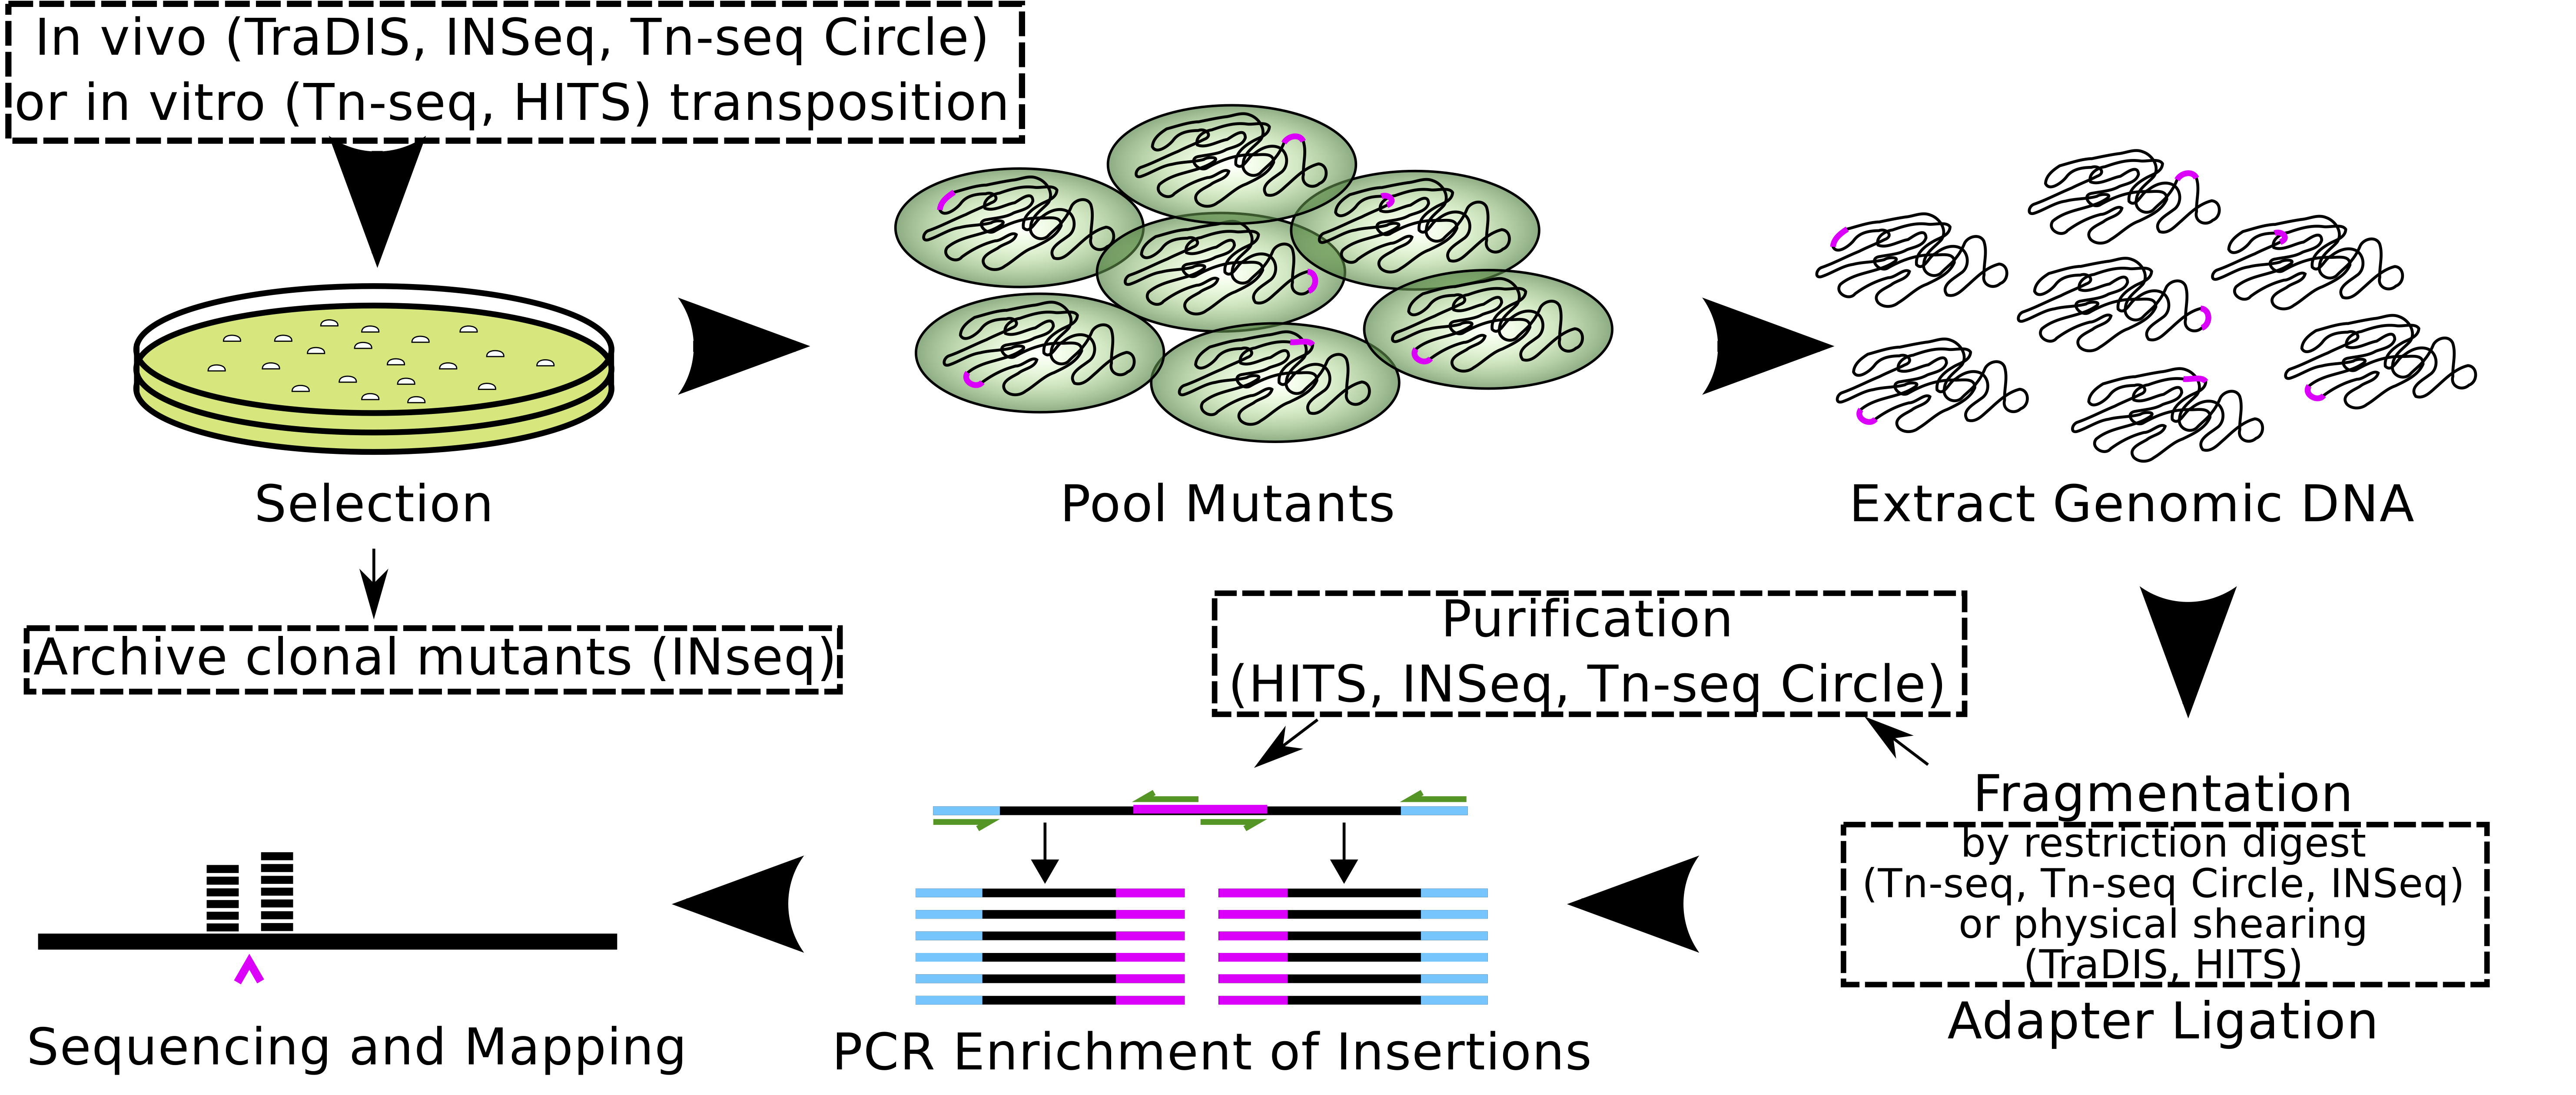
\includegraphics[width=14cm]{protocols}
\caption[Transposon-insertion sequencing protocols]{\textbf{Transposon-insertion sequencing protocols.} An illustration of the workflow typical of transposon-insertion sequencing protocols. Transposons are represented by pink lines, sequencing adaptors by blue, genomic DNA by black, and PCR primers by green. Mutants are generated through either {\it in vivo} or {\it in vitro} transposition and subsequent selection for antibiotic resistance. These mutants are pooled, and optionally competed in test conditions, then genomic DNA is extracted and fragmented by restriction digest or physical shearing. Sequencing adaptors are ligated, some protocols then perform a step to purify fragments containing transposon insertions, and PCR with transposon- and adapter-specific primers is used to specifically enrich for transposon-containing fragments. The fragments are then sequenced and mapped back to a reference genome to uniquely identify insertion sites with nucleotide-resolution. Dashed boxes indicate steps which differ between protocols.
} 
 \label{fig:protocols}
\end{center}
\end{figure}

\subsection{Transposon mutagenesis}
Most studies have used either Tn{\it 5} or Mariner transposon derivatives. Tn{\it 5} originated as a bacterial transposon which has been adapted for laboratory use. Large-scale studies have shown that Tn{\it 5}, while not showing any strong preference for regional GC-content, does have a weak preference for a particular insertion motif \parencite{Shevchenko2002,Adey2010,Green2012}. Transposon-insertion sequencing studies performed with Tn{\it 5} transposons in {\it S}. enterica serovars have reported a slight bias towards AT-rich sequence regions \parencite{Langridge2009a, Barquist2013a}. However, this preference does not appear to be a major obstacle to analysis given the extremely high insertion densities obtained with this transposon \parencite{Langridge2009a, Christen2011, Barquist2013a} (see Table \ref{tab:studies}). Additionally, Tn{\it 5} has been shown to be active in a wide range of bacterial species, though the number of transformants obtained can vary significantly depending on the transformation efficiency of the host. 

Mariner {\it Himar1} transposons on the other hand originate from eukaryotic hosts and have an absolute requirement for TA bases at their integration site \parencite{Lampe1998, Rubin1999}, with no other known bias besides a possible preference for bent DNA \parencite{Lampe1998}. This can be a disadvantage in that it limits the number of potential insertion sites, particularly in GC-rich sequence. However, this specificity can also be used in the prediction of gene essentiality in near-saturated libraries: as every potential integration site is known and the probability of integration at any particular site can be assumed to be roughly equal, it is straight-forward to calculate the probability that any particular region lacks insertions by chance. {\it Himar1} transposition can also be conducted {\it in vitro} in the absence of any host factors \parencite{Lampe1996}, and inserted transposons can then be transferred to the genomes of naturally transformable bacteria through homologous recombination \parencite{Johnsborg2007}. This can be advantageous when working with naturally transformable bacteria with poor electroporation efficiency \parencite{Gawronski2009,Opijnen2009}. It is worth noting that Tn{\it 5} is also capable of transposition {\it in vitro} \parencite{Goryshin1998}, and could potentially be used to increase insertion density and hence the resolution of the assay, particularly in GC-rich genomic regions.

\subsection{Pool construction}

Once mutants have been constructed, they are plated on an appropriate selective media for the transposon chosen, and colonies are counted, picked, and pooled. A disadvantage of this is that the mutants must be recreated for follow up or validation studies. Goodman et al. introduced a clever way around this in the INSeq protocol: by individually archiving mutants, then sequencing combinatorial mutant pools it is possible to uniquely characterize $2n$ insertion mutants by sequencing only $n$ pools \parencite{Goodman2009}. Each mutant is labelled with a unique binary string that indicates which pools it has been added to. These binary strings can then be reconstructed for each insertion observed in these pools by recording their presence or absence in sequencing data, providing a unique pattern relating insertions to archived mutants. The authors control false identifications due to errors in sequencing by requiring that each binary label have a minimum edit distance to every other label, allowing for a robust association of labels with insertions despite sometimes noisy sequencing data. As a proof of concept, the authors were able to identify over 7,000 {\it Bacteroides thetaiotaomicron} mutants from only 24 sequenced pools. This effectively uses methods for the generation of random transposon pools to rapidly generate defined mutant arrays, though it is heavily dependent on liquid-handling robotics.

\subsection{Enrichment of transposon-insertion junctions}

Once pools have been constructed they are grown in either selective or permissive conditions, depending on the experiment, and then genomic DNA is extracted. Fragmentation proceeds either through restriction digestion in the case of transposons modified to contain appropriate sites \parencite{Goodman2009,Opijnen2009, Gallagher2011} or via physical shearing \parencite{Langridge2009a, Gawronski2009}, then sequencing adapters are ligated to the resulting fragments. PCR is performed on these fragments using a transposon-specific primer and a sequencing adapter-specific primer to enrich for fragments spanning the transposon-genomic DNA junction. 

Some protocols purify fragments containing transposon insertions using biotinylated primers \parencite{Gallagher2011, Goodman2011} or PAGE\nomenclature[Z]{PAGE}{Polyacrylamide gel electrophoresis} \parencite{Goodman2009} before and/or after PCR enrichment. The purification step from the Tn-seq Circle protocol is particularly unusual in that restriction digested fragments containing transposon sequence are circularized before being treated with an exonuclease that digests all fragments without transposon insertions, theoretically completely eliminating background \parencite{Gallagher2011}. Given the success of protocols that do not include a purification step and the lack of systematic comparisons, it is currently unclear whether including one provides any major advantages.

\subsection{Sequencing}

The protocol steps described so far are broadly similar to those used in microarray-based studies of transposon mutant pools. The major advancement that has driven transposon-insertion sequencing has been the recent development of second generation DNA sequencing technologies. For 30 years, DNA sequencing was dominated by dideoxynucleotide, or Sanger, sequencing, first described by \textcite{Sanger1977}. Sanger sequencing requires a clonal population of template DNA molecules, to which a primer and a full complement of four deoxynucleotides (dNTPs\nomenclature[Z]{dNTP}{deoxynucleotide}) and a single species of dideoxynucleotide (ddNTP\nomenclature[Z]{ddNTP}{dideoxynucletoide}) are added. DNA polymerase is then used to perform rounds of DNA extension, with ddNTPs stochastically terminating the reaction, before the resulting fragments are denatured and separated with gel electrophoresis. By running four such reactions with each species of ddNTP, the sequence of the template molecule can be determined by reading off bands on the gel. A number of advancements progressively improved the throughput and decreased the cost of Sanger sequencing, including the substitution of capillary electrophoresis for gel electrophoresis and the use of fluorescently labelled ddNTP (fluorescent dye-terminator sequencing) enabling sequencing in a single reaction. However, even with these advances the throughput of Sanger sequencing remained in the range of kilobases of sequence per hour, and costs remained high due to requirements for template cloning and inherent limitations in the technology \parencite{Morozova2008}.

The development of second generation sequencing technologies in the early-mid 2000's broke these barriers to the adoption of sequencing as a routine experimental technique. These technologies include Roche 454 pyrosequencing, Illumina/Solexa reversible terminator sequencing, and ABI SOLiD parallel sequencing by ligation. While in principle any of these technologies could be applicable to transposon-insertion sequencing, all studies to date have used Solexa sequencing. Solexa sequencing is similar in principle to Sanger sequencing, with two major innovations: the ability to generate arrayed clonal clusters of template molecules on a glass flow cell (described by \textcite{Fedurco2006}) allowing for hundreds of thousands of simultaneous sequencing reactions, and the adoption of reversible dye terminator chemistry (described by \textcite{Bentley2008}) which allows for fluorescently labelled terminators to be rapidly stripped of their fluorophore, their termination reversed, and extension continued. By monitoring successive rounds of these hundreds of thousands of parallel sequencing reactions with a CCD\nomenclature[Z]{CCD}{Charge-coupled device} camera, the sequence of a large population of template molecules can be determined quickly and simultaneously, leading to current throughputs of megabases to gigabases of sequence per hour. As each resulting read corresponds to a single template molecule, this technology is ideally suited to monitoring populations of transposon mutants, providing an accurate digital count of insertion prevalence.

\section{Reproducibility, accuracy, and concordance with previous methods}

A number of studies have looked at the reproducibility of transposon-insertion sequencing. Multiple studies using different protocol variations have repeatedly shown extremely high reproducibility in the number of insertions per gene (correlations of ~90\%) in replicates of the same library grown and sequenced independently \parencite{Goodman2009, Opijnen2009, Gallagher2011}, and good reproducibility (correlations between 70-90\%) in independently constructed unsaturated libraries \parencite{Opijnen2009,Opijnen2012}. \Textcite{Opijnen2012} compared traditional 1 X 1 competition experiments between wild-type and mutant {\it Streptococcus pneumoniae} to results obtained by transposon-insertion sequencing and showed that there was no significant difference in results over a range of tested conditions. The accuracy of transposon-insertion sequencing in determining library composition has also been assessed. \Textcite{Zhang2012} constructed a library of identified transposon-insertion mutants in known relative quantities, and then were able to recover the relative mutant prevalence with transposon-insertion sequencing. Additionally, by estimating the number of PCR templates prior to enrichment, this study showed that there is a high correlation between enrichment input and sequencing output. 

Two studies have evaluated concordance between results obtained with transposon-insertion sequencing and microarray monitoring of transposon insertions in order to demonstrate the enhanced accuracy and dynamic range of sequencing over previous methods. In the first, 19 libraries of 95 enterohemorrhagic {\it Escherichia coli} (EHEC)\nomenclature[Z]{EHEC}{Enterohemorrhagic {\it Escherichia coli}} transposon mutants that had previously been screened in cattle using signature-tagged mutagenesis (STM)\nomenclature[Z]{STM}{Signature-tagged mutagenesis} were pooled and re-evaluated using the TraDIS protocol \parencite{Eckert2011}. The original STM study had identified 13 insertions in 11 genes attenuating intestinal colonization in a type III secretion system located in the locus of enterocyte effacement (LEE)\nomenclature[Z]{LEE}{Locus of enterocyte effacement} \parencite{Dziva2004}. By applying sequencing to the same samples, an additional 41 mutations in the LEE were identified, spanning a total of 21 genes. Additional loci outside the LEE which have been previously implicated in intestinal colonization but had not been detected by STM were also reported by TraDIS. 

The second study re-evaluated genes required for optimal growth determined by TraSH in {\it Mycobacterium tuberculosis} \parencite{Sassetti2003, Griffin2011}. The greater dynamic range of sequencing as compared to microarrays allowed easier discrimination between insertions that were truly unviable and those that were only significantly underrepresented. The authors estimate that genes called as required by sequencing in their study are at least 100-fold underrepresented in the pool. In comparison, the threshold in the previous microarray experiment reported genes that had log probe ratios at least 5-fold lower than average between transposon-flanking DNA hybridization and whole genomic DNA hybridization. Additionally, the nucleotide-resolution of insertion sequencing allowed the authors to identify genes which had required regions, likely corresponding to required protein domains \parencite{Zhang2012}, but which tolerated insertions in other regions.  Altogether the authors increase the set of genes predicted to be required for growth in laboratory conditions in {\it M. tuberculosis} by more than 25\% (from 614 to 774).

\section{Identifying gene requirements}

\subsection{Gene essentiality}

The study of gene essentiality has its roots in evolutionary theory, systems biology, and comparative genomics, and has been instrumental in the development of the emerging discipline of synthetic biology. Koonin summarizes the major scientific motivation behind this line of research succinctly: ``When reverse-engineering a complex machine, one basic goal is to draw up a list of essential parts'' \parencite{Koonin2003}. The earliest attempt at constructing such a minimal gene set involved a comparison between the first two complete genomes sequenced: {\it M. genitalium} and {\it Haemophilus influenzae} \parencite{Mushegian1996}. Both of these organisms are pathogens with highly reduced genomes; however, they are derived from distant branches of the bacterial phylogeny being Gram-positive and -negative, respectively. Orthology prediction based on sequence similarity identified 240 genes shared between the two organisms. However, a number of essential pathways were found to be incomplete in this set due to non-orthologous gene displacement (NOGD)\nomenclature[Z]{NOGD}{Nonorthologous gene displacement}, and a true minimal gene set was estimated to contain 256 genes. NOGD apparently occurs when an unrelated but functionally analogous gene is introduced in a lineage, and subsequently the ancestral gene is lost. The sequencing of complete genomes has shown that this phenomena is surprisingly wide-spread, and only $\sim$60 genes appear to be universally conserved \parencite{Koonin2003}. Rather obviously in hindsight, it appears that gene essentiality is highly dependent on the evolutionary and systems context in which the gene occurs - our essential parts list depends on the machine we wish to build.

Large-scale experimental studies seem to confirm this. A range of approaches have been taken to experimentally determining the `essential' genes of a diverse array of organisms. These include plasmid-insertion mutagenesis in {\it Bacillus subtilis} \parencite{Kobayashi2003}, antisense-mediated gene inactivation in {\it H. influenzae} \parencite{Akerley2002}, transposon mutagenesis in {\it Pseudomonas aerguinosa} \parencite{Jacobs2003}, and insertion-duplication mutagenesis in {\it S. enterica} \parencite{Knuth2004}. However, the ``gold standard'' for the determination of gene essentiality is repeated failure to generate targeted single gene deletions. Comprehensive single gene deletion libraries libraries have been created for the $\gamma$-proteobacteria {\it E. coli} and {\it Acinetobacter baylyi} \parencite{Baba2006, Berardinis2008} where $\lambda$-red mediated recombineering has simplified the generation of defined deletions \parencite{Datsenko2000}, though the process is still extremely labor-intensive. Typical estimates for essential gene sets determined by these various techniques range from less than 300 to 600 genes, depending on the organism. This variability is likely dependent on a variety of factors, including false positives and negatives due to experimental techniques, the growth conditions of the experiment, intrinsic properties of the cell being manipulated, and accidents of evolution. Now that it has become feasible to synthesize a viable bacterial chromosome \parencite{Gibson2010}, a deeper understanding of the factors affecting gene essentiality is the next hurdle on the road to engineering truly synthetic life.

\subsection{Applications of transposon-insertion sequencing}

The earliest application of transposon-insertion sequencing, and indeed the earliest experimental study of gene essentiality, was to determine the minimal set of genes necessary for the survival of {\it Mycoplasma} \parencite{Hutchison1999}. This essential genome is of great interest in synthetic and systems biology where it is seen as a foundation for engineering cell metabolism as described previously, and also in infection biology and medicine where it is seen as a promising target for therapies. However, it is important to remember that �essentiality� is always relative to growth conditions: a biosynthetic gene that is non-essential in a growth medium supplying a particular nutrient may become essential in a medium that lacks it. Traditionally, gene essentiality has been determined in clonal populations \parencite{Baba2006, Jacobs2003, Glass2006}; since the high-throughput transposon sequencing protocols described here necessarily contain a short period of competitive growth before DNA extraction, many of these studies prefer to refer to the �required� genome for the particular conditions under evaluation. 

Because of this short period of competitive growth, and because many otherwise required genes tolerate insertions in their terminus \parencite{Goodman2009, Griffin2011, Zomer2012} or outside essential domains \parencite{Zhang2012} the determination of required genomic regions is not completely straight-forward and a number of approaches have been taken to counter this. These include only calling genes completely lacking insertions as required \parencite{Opijnen2009}, or determining a cut-off based on the empirical or theoretical distribution of gene-wise insertion densities \parencite{Langridge2009a,Barquist2013a, Griffin2011, Zomer2012}. Additionally, windowed methods have been developed which can be used to identify essential regions in the absence of gene annotation \parencite{Zhang2012, Dejesus2013}, and have had success in identifying required protein domains, promoter regions, and non-coding RNAs\nomenclature[Z]{RNA}{Ribonucleic acid} (ncRNAs)\nomenclature[Z]{ncRNA}{non-coding RNA}. The organisms that have been evaluated for gene requirements under standard laboratory conditions are summarized in Table \ref{tab:studies}. In agreement with previous studies \parencite{Baba2006, Jacobs2003}, many required genes identified by transposon-insertion sequencing are involved in fundamental biological processes such as cell division, DNA replication, transcription and translation \parencite{Langridge2009a, Goodman2009, Barquist2013a, Griffin2011}, and many of these requirements appear to be conserved between genera and classes \parencite{Barquist2013a,Christen2011}. 

However, a recent study defining required gene sets in {\it Salmonella} serovars (described in detail in the next chapter) has found that phage repressors, necessary for maintaining the lysogenic state of the prophage, are also required \parencite{Barquist2013a}, even though mobile genetic elements such as phage are usually considered part of the accessory genome. This study also highlights the need for temperance when interpreting the results of high-throughput assays of gene requirements. For example, many genes in {\it Salmonella} Pathogenicity Island 2 (SPI-2)\nomenclature[Z]{SPI}{{\it Salmonella} pathogenicity island} did not exhibit transposon-insertions, despite clear evidence from directed knockouts showing that these genes are non-essential for viability or growth. Under laboratory conditions, SPI-2 is silenced by the nucleoid-forming protein H-NS \parencite{Lucchini2006,Navarre2006}, which acts by oligermerizing along silenced regions of DNA blocking RNA polymerase access. A previous study has shown that transposon insertion �cold spots� can be caused by competition between high-density proteins and transposases for DNA \parencite{Manna2007}. This suggests that H-NS may be restricting transposase access to DNA, though this has not previously been observed in transposon-insertion sequencing data, and will require additional work to confirm.

\section{Determining conditional gene requirements}

One of the most valuable applications of the transposon-insertion sequencing method is the ability to identify genes important in a condition of interest, by comparing differences in the numbers of sequencing reads from input (control) mutant pools to output (test) pools that have been subject to passaging in a certain growth condition. Insertion counts are compared from cells in the input pool and those after passage, thereby identifying genes that either enhance or detract from survival and/or growth in the given condition, defined by decreased or increased insertion frequency, respectively. I describe a pipeline for analyzing such experiments in chapter {\color{red} XX TraDIS PIPELINE CHAPTER HERE}. A further application of this method involves comparing insertions between biologically linked conditions, such as cellular stresses or different stages of a murine infection, to gain insight into complex systems \parencite{Opijnen2012}.

So far, transposon-insertion sequencing has been used to investigate a number of interesting biologically relevant conditions: bile tolerance in {\it S.} Typhi \parencite{Langridge2009a} and {\it S.} Typhimurium \parencite{Khatiwara2012}, bacteriophage infection of {\it S.} Typhi \parencite{Pickard2013}, antibiotic resistance in {\it P. aeruginosa} \parencite{Gallagher2011}, cholesterol utilization in {\it M. tuberculosis} \parencite{Griffin2011} and survival in number of stress and nutrient conditions in {\it S. pneumoniae} \parencite{Opijnen2012}. Transposon-insertion sequencing of populations passed through murine models have been used to assess genes required to establish the gut commensal {\it B. thetaiotaomicron} in its niche \parencite{Goodman2009}, for {\it H. influenzae} infection \parencite{Gawronski2009}, as well as {\it S. pneumoniae} responses to two {\it in vivo} niches - the lung and nasopharynx \parencite{Opijnen2012}. A further extension of the method examined double mutant libraries, that is transposon mutant libraries generated in a defined deletion background, to tease apart complex networks of regulatory genes \parencite{Opijnen2009}.

Two studies in particular illustrate the power of using transposon-insertion sequencing to identify conditionally required genes. In the first, \textcite{Goodman2009} set out to determine the genes necessary for the establishment of the commensal {\it B. thetaiotaomicron} in a murine model. First, the growth requirements of transposon mutant populations in the cecum of germ-free mice was assessed, and genes required for growth in monoassociation with the host were found to be enriched in functions such as energy production and amino acid metabolism. By further comparing monoassociated transposon mutant libraries with those grown in the presence of three defined communities of human gut-associated bacteria, the authors identified a locus up-regulated by low levels of vitamin B12 that is only required in the absence of other bacteria capable of synthesizing B12. This showed that the gene requirements of any particular bacterium in the gut are at least partially dependent on the metabolic capabilities of the entire community and emphasizes the importance of testing {\it in vivo} conditions to complement {\it in vitro} study.

The second study, conducted by \textcite{Opijnen2012}, aimed to map the genetic networks involved in a range of cellular stress responses in {\it S. pneumoniae}. Seventeen {\it in vitro} conditions were tested, including: pH, nutrient limitation, temperature, antibiotic, heavy metal, and hydrogen peroxide stress. Approximately 6\% of disrupted genes resulted in increased fitness in some condition, suggesting that some genes are maintained despite being detrimental to the organism under particular conditions. These would be interesting candidates for further functional and evolutionary study, as the maintenance of these genes is presumably highly dependent on the conditions the bacteria faces, and may have implications for our understanding of e.g. gene loss in the process of bacterial host adaptation \parencite{Toft2010}. Two additional {\it in vivo} experiments were performed in a murine model, where cells were recovered from the lung and nasopharynx. Combining this data, over 1,800 genotype-phenotype genetic interactions were identified. These interactions were mapped and pathways identified. Between the two {\it in vivo} niches, certain stress responses pathways were markedly different. For example, temperature stress produced a distinct response in the lung, compared to the nasopharyanx, which is perhaps to be expected as temperature varies greatly between these two sites. By further examining sub-pathways required in the two different niches and comparing them to {\it in vitro} requirements, the authors were able to draw conclusions regarding the condition {\it S. pneumoniae} faces when establishing an infection. This comprehensive mapping of genotype-phenotype relationships will serve as an important atlas for further studies of the factors affecting {\it S. pneumoniae} carriage and virulence.

\section{Monitoring ncRNA contributions to fitness}

To date, four studies (including one described in detail in the next chapter) have used transposon-insertion sequencing to examine the contribution of non-coding RNAs (ncRNAs) and other non-coding regions to organismal fitness (see Table \ref{tab:studies}). Two of these examined requirements for non-coding regions in the relatively under-explored bacterial species {\it Caulobacter crescentus} \parencite{Christen2011} and {\it M. tuberculosis} \parencite{Zhang2012}. Both utilized analytical techniques that allowed for the identification of putative required regions in the absence of genome annotation. Twenty-seven small RNAs (sRNAs)\nomenclature[Z]{sRNA}{Bacterial small RNA} had previously been detected in {\it C. crescentus} \parencite{Landt2008}; 6 were found to be depleted in transposon insertions indicating an important role in basic cellular processes. Additionally, the well-characterized ncRNAs tmRNA\nomenclature[Z]{tmRNA}{Transfer-messenger RNA} and RNase\nomenclature[Z]{RNase}{Ribonuclease} P, as well as 29 non-redundant tRNAs\nomenclature[Z]{tRNA}{Transfer RNA} were found to be required. An additional 90 unannotated non-disruptable regions were identified throughout the genome, implying an abundance of unexplored functional non-coding sequence. 

\begin{figure}[htp]
\begin{center}
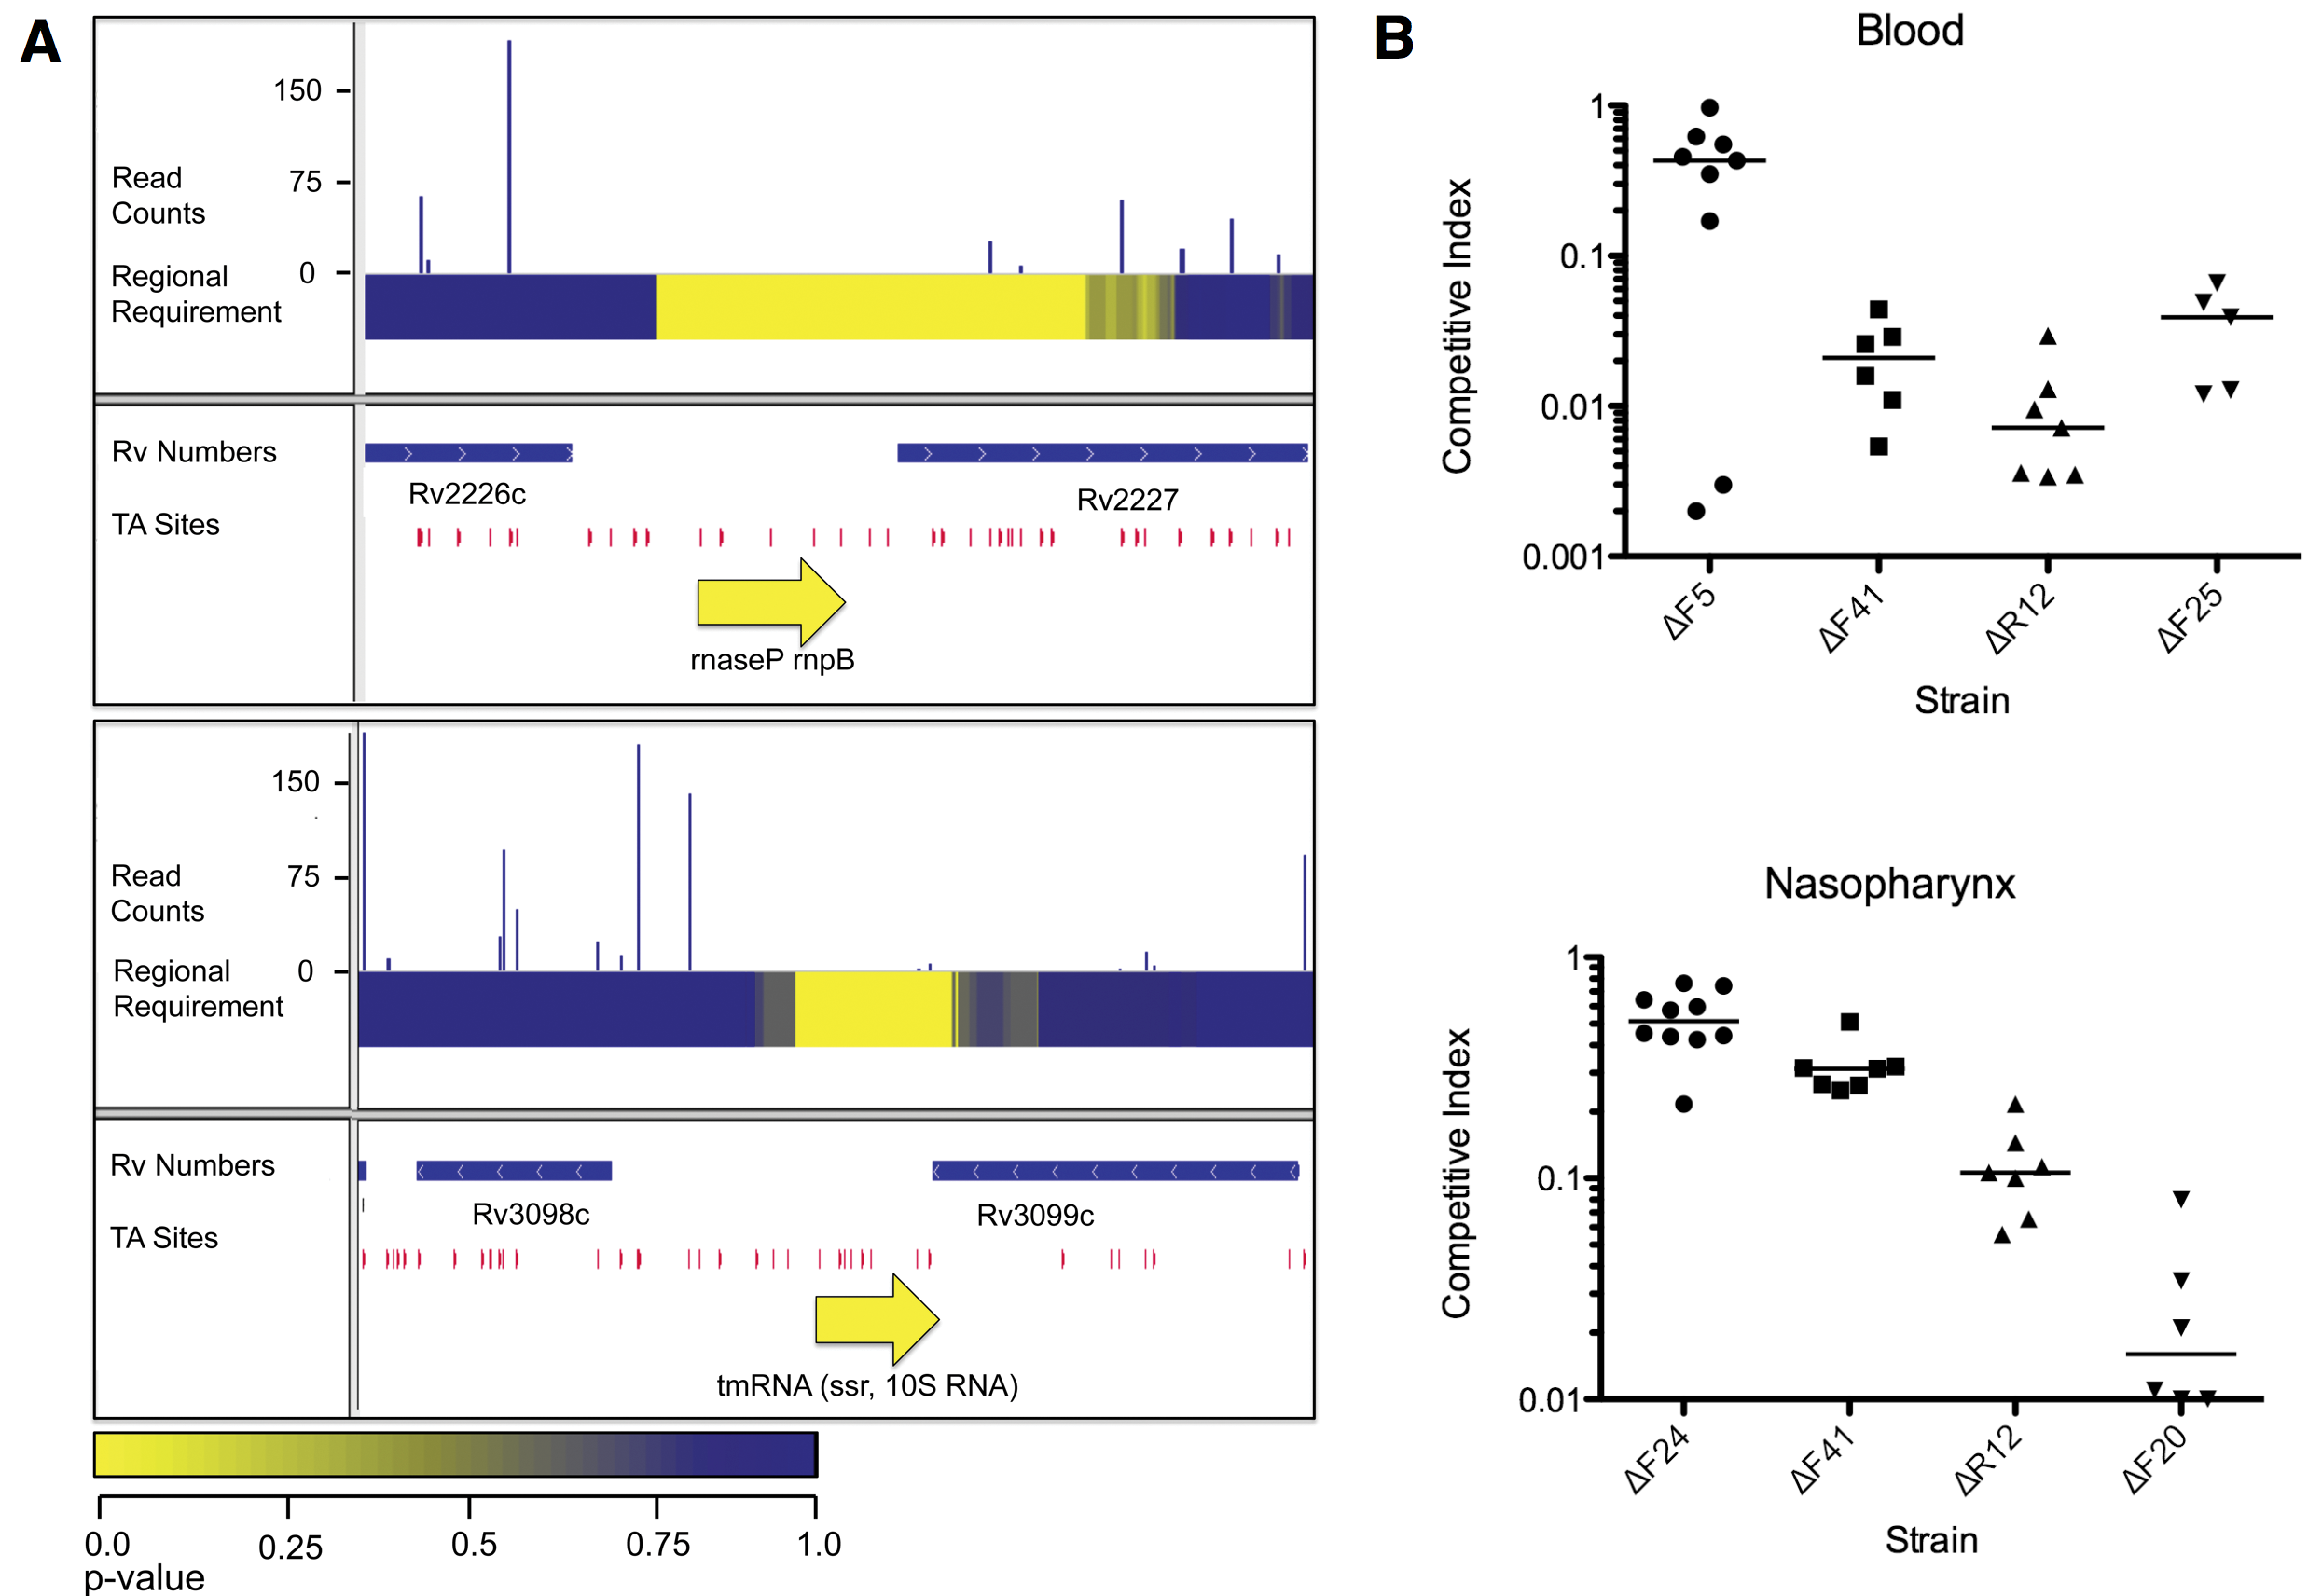
\includegraphics[width=14cm]{ncrnas.png}
\caption[Applications of transposon-insertion sequencing to non-coding RNAs]{\textbf{Applications of transposon-insertion sequencing to non-coding RNAs.} A) Plots of genomic regions in {\it Mycobacterium tuberculosis} containing the required non-coding RNAs RNase P (top) and tmRNA (bottom). Tracks, from top to bottom: 1. Histogram of insertion counts, 2. Comprehensive heat-map of requirement of 500-bp\nomenclature[Z]{bp}{Base pair} windows, 3. Position of annotated genes, 4. Position of TA dinucleotide sites, 5. Position of non-coding RNA. Reproduced from \textcite{Zhang2012}. B) 1 X 1 competition assays validate attenuating {\it Streptococcus pneumoniae} sRNA mutants identified by transposon-insertion sequencing. Mice were infected with defined deletions of sRNAs identified as attenuating by Tn-seq and wild type {\it S. pneumoniae} TIGR4 at the body site indicated and bacterial densities were compared 24 hours post-infection. These plots show the derived competitive index in blood (top) and the nasopharnyx (bottom). Each point represents the result of a competition experiment between an sRNA deletion mutant and wild-type TIGR4. A competitive index of 1 indicates equivalent numbers of mutants and wild-type were recovered. Modified from \textcite{Mann2012}.
} 
\label{fig:ncrnas}
\end{center}
\end{figure}

While the non-coding transcripts of {\it M. tuberculosis} have been explored more thoroughly than those of {\it C. crescentus}, most remain functionally uncharacterized, though there are hints that some of these may be involved in pathogenicity \parencite{Arnvig2012}. Using a Mariner transposon-based assay and a windowed statistical analysis that accounted for the distribution of potential TA integration sites, 35 intergenic regions were identified as putatively required in the {\it M. tuberculosis} genome \parencite{Zhang2012}.  In common with the {\it C. crescentus} study, the RNA component of RNase P, required for the maturation of tRNAs, and tmRNA, involved in the freeing of stalled ribosomes, were identified as required (Figure \ref{fig:ncrnas} A) together with 10 non-redundant tRNAs and potential promoter regions. However, due to the lower overall insertion density and lack of TA sites in some GC-rich regions, there were some regions that could not be assayed and the resolution was limited to 250 bases.

A particularly exciting study has been conducted in {\it S. pneumoniae} TIGR4 combining RNA-seq\nomenclature[Z]{RNA-seq}{RNA sequencing} with transposon-insertion sequencing \parencite{Mann2012}. To identify sRNA loci the authors first sequenced size-select RNA from wild type TIGR4 and three two-component system knockouts, identifying 89 putative sRNAs, 56 of which were novel. Fifteen of these candidates, selected on the basis of high expression and low predicted folding free energy, were assayed for their ability to establish invasive disease in a murine model. Of these 8 sRNA deletions showed a significant attenuation of disease. To more broadly establish the roles of sRNAs in infecting particular organs, transposon insertion libraries were administered directly to the nasopharnyx, lungs, or blood of mice, and bacteria were harvested following disease progression. Twenty-six, 28, and 18 sRNAs were found to attenuate infection in the nasopharnyx, lung and blood respectively. These results were then validated with targeted deletions of 11 sRNAs (Figure  \ref{fig:ncrnas} B). In addition to establishing the role of sRNAs in {\it S. pneumoniae} virulence, this study illustrated the power of combining RNA-seq and transposon-insertion sequencing to rapidly assign phenotypes to non-coding sequences.

\section{Limitations}

In this chapter, I have largely focused on the potential of transposon insertion sequencing. However, this technology does have a number of important limitations. As discussed previously, requirements for particular nucleotides at insertion sites, such as the TA required by Mariner transposons, or preference for certain sequence composition, such as the AT bias exhibited by Tn{\it 5}, can limit the density of observed insertions in certain genomic regions. This may impact any down-stream analysis, and can potentially bias results, particularly the determination of gene requirements. Even if this bias has been accounted for, transposon-insertion screens will always over-predict gene requirements in comparison to targeted deletion libraries as discussed previously. However, this over-prediction can be controlled either through careful consideration of known insertion biases as in many Mariner-based studies, or by high insertion densities, such as those achieved in several Tn{\it 5}-based studies (Table \ref{tab:studies}). Once the library has been created, only regions that have accumulated insertions in the conditions of library creation will be able to be assayed for fitness effects in further conditions. This means that regions that lead to slow growth phenotypes when disrupted in standard laboratory conditions may be difficult to assay in other conditions. Additionally, the dynamic range of fitness effects detected will depend on the complexity of the input library(s). The absence of insertions may be a particular problem for assaying small genomic elements, such as sRNAs or short ORFs\nomenclature[Z]{ORF}{Open reading frame}. Finally, the validation of hypotheses derived from transposon-insertion sequencing will require the construction of targeted deletions, as individual mutants cannot be recovered from pools unless specialized protocols have been followed during library construction (as in \cite{Goodman2009}).

\section{The future of transposon-insertion sequencing}

Transposon-insertion sequencing is a robust and powerful technique for the rapid connection of genotype to phenotype in a wide range of bacterial species. Already, a number of studies have demonstrated the effectiveness of this method and the results have been far-reaching: enhancing our understanding of basic gene functions, establishing requirements for colonization and infection, mapping complex metabolic pathways, and exploring non-coding genomic �dark matter�. Due to the range of potential applications of transposon-insertion sequencing, along with the decreasing cost and growing accessibility of next-generation sequencing, I believe that this method will become increasingly common in the near future. 

A number of bacterial species have already been subjected to transposon-insertion sequencing (Table \ref{tab:studies}). Microarray-based approaches to monitoring transposon mutant libraries have even been applied to eukaryotic systems \parencite{Ross-Macdonald1999}, and similarly transposon-insertion sequencing can potentially be applied to any system where the creation of large-scale transposon mutant libraries is technologically feasible. Recently the Genomic Encyclopedia of Bacteria and Archea (GEBA)\nomenclature[Z]{GEBA}{Genomic encyclopedia of bacteria and archea} \parencite{Wu2009} has been expanding our knowledge of bacterial diversity through targeted genomic sequencing of underexplored branches of the tree of life. Applying transposon-insertion sequencing in a comparative manner across the bacterial phylogeny will provide an unprecedented view of the determinants for survival in diverse environments - the next chapter describes a study taking the first steps toward this eventual goal \parencite{Barquist2013a}. While most transposon-insertion sequencing studies to date have focused on pathogenic bacteria, these techniques could also have applications in energy production, bioremediation, and synthetic biology.

The combination of transposon-insertion sequencing with other high-throughput and computational methods is already proving to be fertile ground for enhancing our understanding of bacterial systems. For instance, by using transposon-insertion sequencing in a collection of relatively simple conditions combined with a computational pathway analysis, \textcite{Opijnen2012} were able to provide a holistic understanding of the genetic subsystems involved in a complex process such as {\it S. pneumoniae} pathogenesis. In the future, methods to assay phenotype in a high-throughput manner (\cite{Bochner2009,Nichols2011}; See also chapter {\color{red} XX BIOLOG CHAPTER HERE}) may be combined with transposon-insertion sequencing to provide exhaustive simple genotype-phenotype associations with which to understand complex processes in a systems biology framework. I look forward to the adoption of these data sets by the community as an important tool for rapid hypothesis generation.

% ------------------------------------------------------------------------


%%% Local Variables: 
%%% mode: latex
%%% TeX-master: "../thesis"
%%% End: 


